%----------------------------------------
% Preamble to set up the document
%----------------------------------------
\documentclass{article}

% set up packages (you shouldn't need to touch this)
\usepackage{graphicx}  % required to insert images
\usepackage{listings}
\usepackage{hyperref}  % for hyperlinks
\usepackage{float}
\usepackage[svgnames]{xcolor}  % to change hyperlink colors
\graphicspath{ {img/} }
\colorlet{linkcolour}{DarkBlue}
\hypersetup{colorlinks=true, linkcolor=linkcolour, citecolor=linkcolour, urlcolor=linkcolour,}

% Margins
\topmargin=-0.45in
\evensidemargin=0in
\oddsidemargin=0in
\textwidth=6.5in
\textheight=9.0in
\headsep=0.25in

% use a sans serif font
\renewcommand{\familydefault}{\sfdefault}

%----------------------------------------
% Step 1: Edit the lecture title
%----------------------------------------
\title{
Lecture 1: Introduction / Overview \\  % Lecture title
Modeling Social Data, Spring 2019 \\   % Course title
Columbia University                    % School
}

%----------------------------------------
% Step 2: Edit your name and the date
%----------------------------------------
\author{Alex Kong}                     % Scribe's name
\date{April 12, 2019}                % Lecture date

\begin{document}

\maketitle


%----------------------------------------
% Step 3:
% Rename uni.tex to match your uni,
% edit the filename accordingly below,
% and put your notes in this file
%----------------------------------------
%----------------------------------------
% Write your notes here
%----------------------------------------
\section{An intro to igraph}

When it comes to graph analysis in R, igraph is a very popular tool.

An example of generating a star graph:

\begin{lstlisting}[language=R]
star <- graph.star(5, mode="undirected", center=1)
plot(star)
get.edgelist(star)
get.adjacency(star)
\end{lstlisting}

Running this code, you'll get a visual representation of the star graph, plus edge and adjacency list representations (remember those?). You'll get a graph looking like this:

\begin{figure}[h]
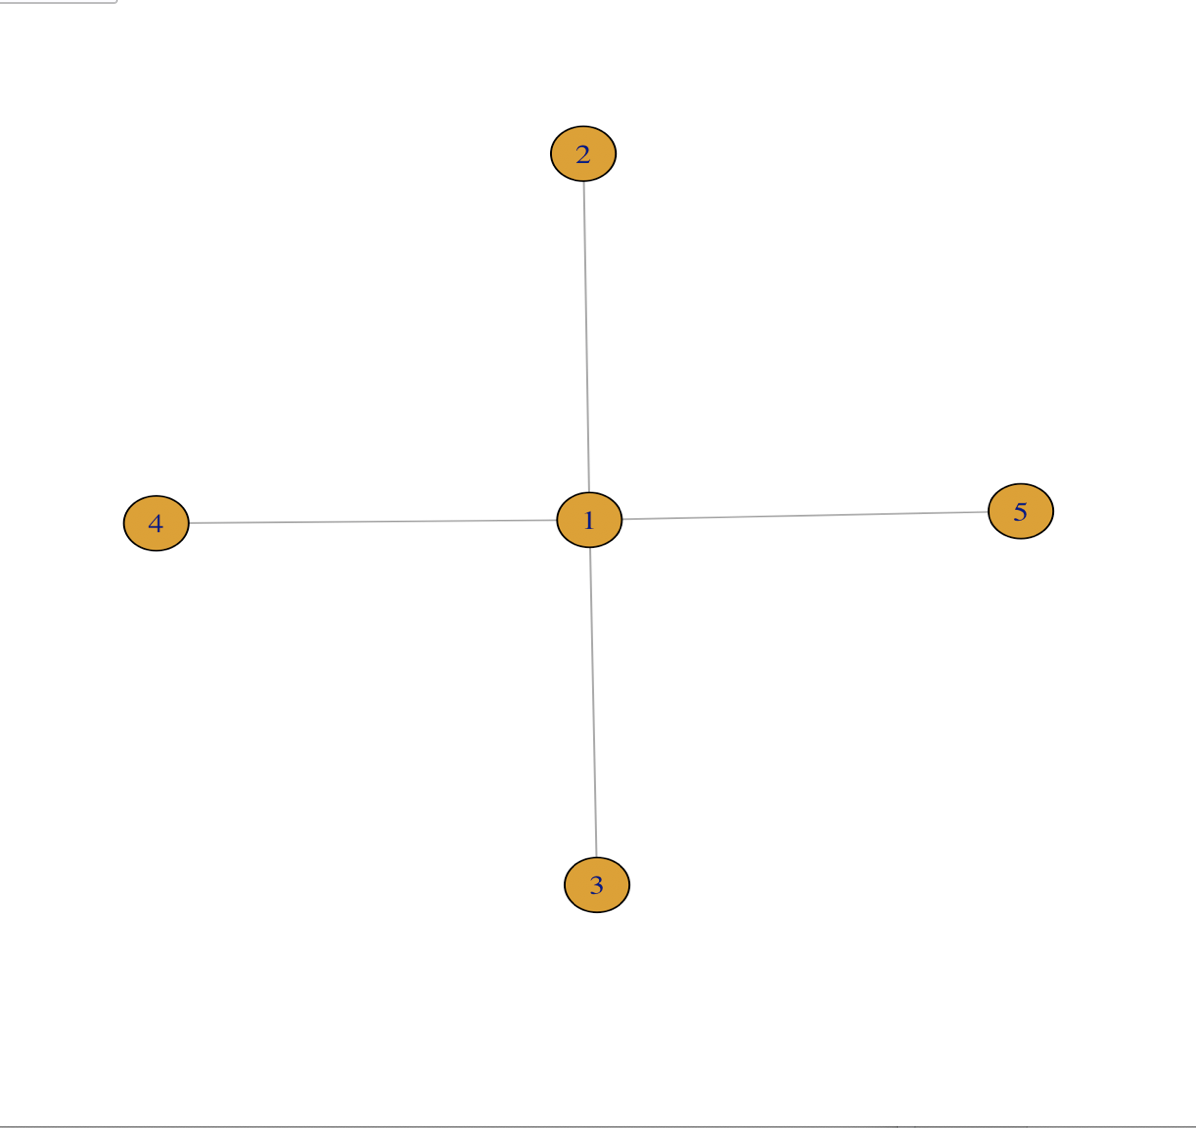
\includegraphics[width=5cm, height=5cm]{figures/star.png}
\centering
\end{figure}

and representations looking like this:

\begin{figure}[h]
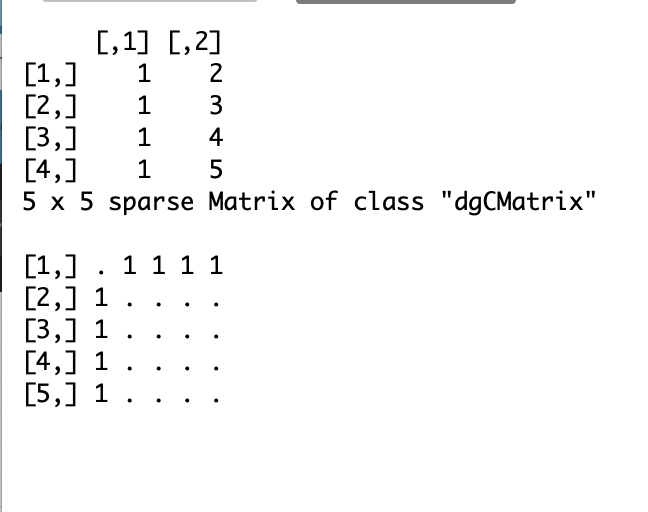
\includegraphics[width=5cm, height=5cm]{figures/graph_rep.png}
\centering
\end{figure}

In case it's not clear, the edge list representation of an igraph is an $|$E$|$ by 2 matrix, where $|$E$|$ is the number of edges and the 2 comes from needing to list both nodes in an edge. The edges are assigned in ascending order based on the node numbering.

Adjacency lists are very intuitive. On a side note, since they often have a lot of unused space, they are represented using a sparse matrix to save memory.

There are other representations such as lattice and ring you can play with as well. One of the more interesting ones worth playing with is the Watts-Strogatz models in watts.strogatz.game. Here's a Wikipedia article explaining more: \href{https://en.wikipedia.org/wiki/Watts\%E2\%80\%93Strogatz_model}{Watts-Strogatz network model}

\section{Using igraph to compute degree distributions}

Degree distributions can tell us a lot of stuff. For example, in friend networks, the greater the degree of a person, the more popular the person could be. And they do more than just tell us things on an individual level. They can teach us important information about entire populations.

Computing degree distribution just requires a little playing around with the tidyverse. We'll show an example using the Wiki degree dist dataset:

\begin{lstlisting}[language=R]
wiki_edges <- read.table('wiki-Vote.txt', sep="\t", header=F, col.names=c('src','dst'))
wiki_graph <- graph.data.frame(wiki_edges, directed=T) # graph representation

wiki_degree_dist <- wiki_edges %>%
  group_by(src) %>% # group by the source node
  summarize(degree=n()) %>% # get the degree of each node
  group_by(degree) %>% # group by the degree
  summarize(num_nodes=n()) # compute how many nodes had a given degree
\end{lstlisting}

We can visualize the degree of the node, one example as follows:

\begin{lstlisting}[language=R]
ggplot(wiki_degree_dist, aes(x = degree, y = num_nodes)) +
  geom_line() + 
  xlab('Degree') +
  ylab('Number of nodes')
\end{lstlisting}

And the resulting plot:

\begin{figure}[h]
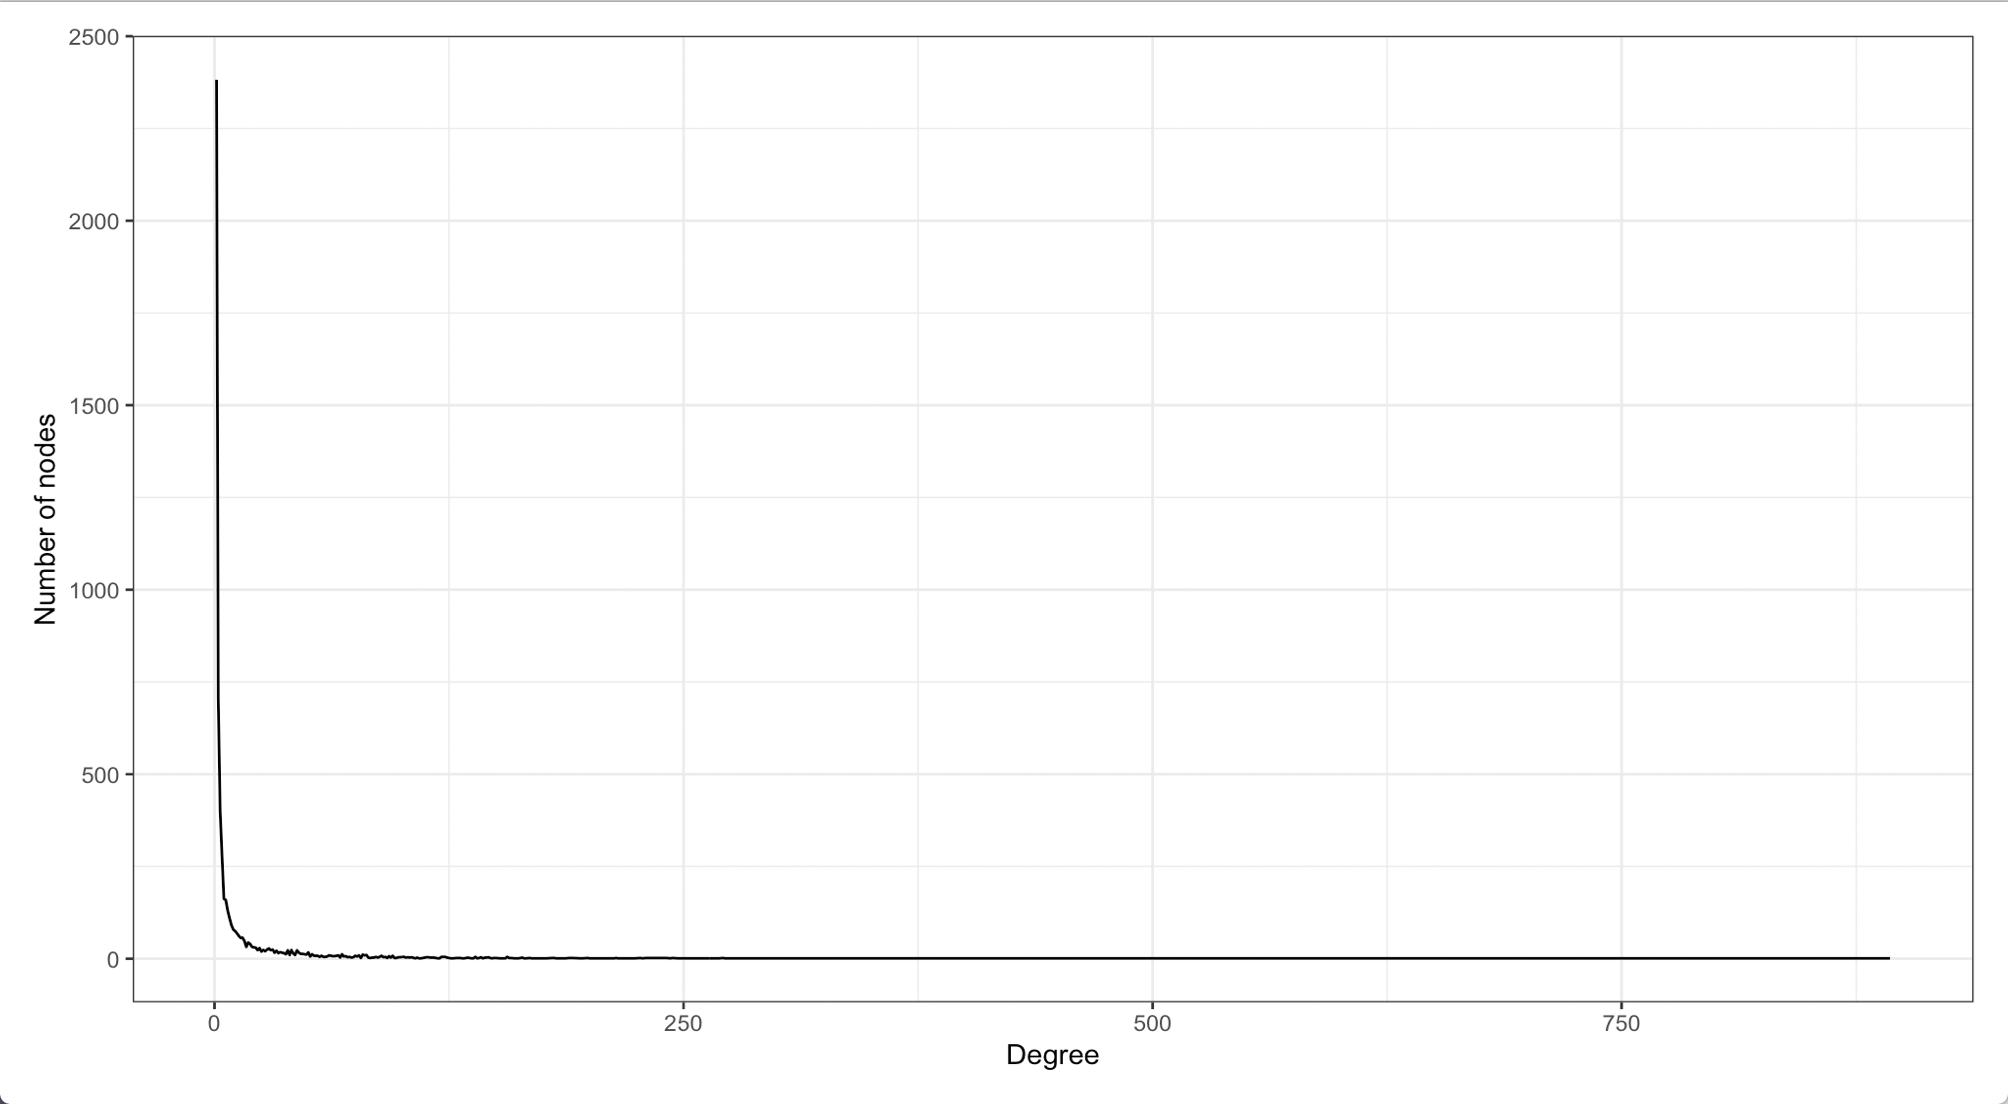
\includegraphics[width=11cm, height=7cm]{figures/node_deg.png}
\centering
\end{figure}

What do you think we can learn based on what we know about Wiki degrees?

igraph also allows one to compute and plot a histogram of the average path length between nodes:

\begin{lstlisting}[language=R]
count <- path.length.hist(wiki_graph)$res
plot_data <- data.frame(path_length = 1:length(count), count)
ggplot(plot_data, aes(x = path_length, y = count)) +
  geom_line() +
  xlab('Path length') +
  ylab('Number of routes')
\end{lstlisting}

and the corresponding plot:

\begin{figure}[h]
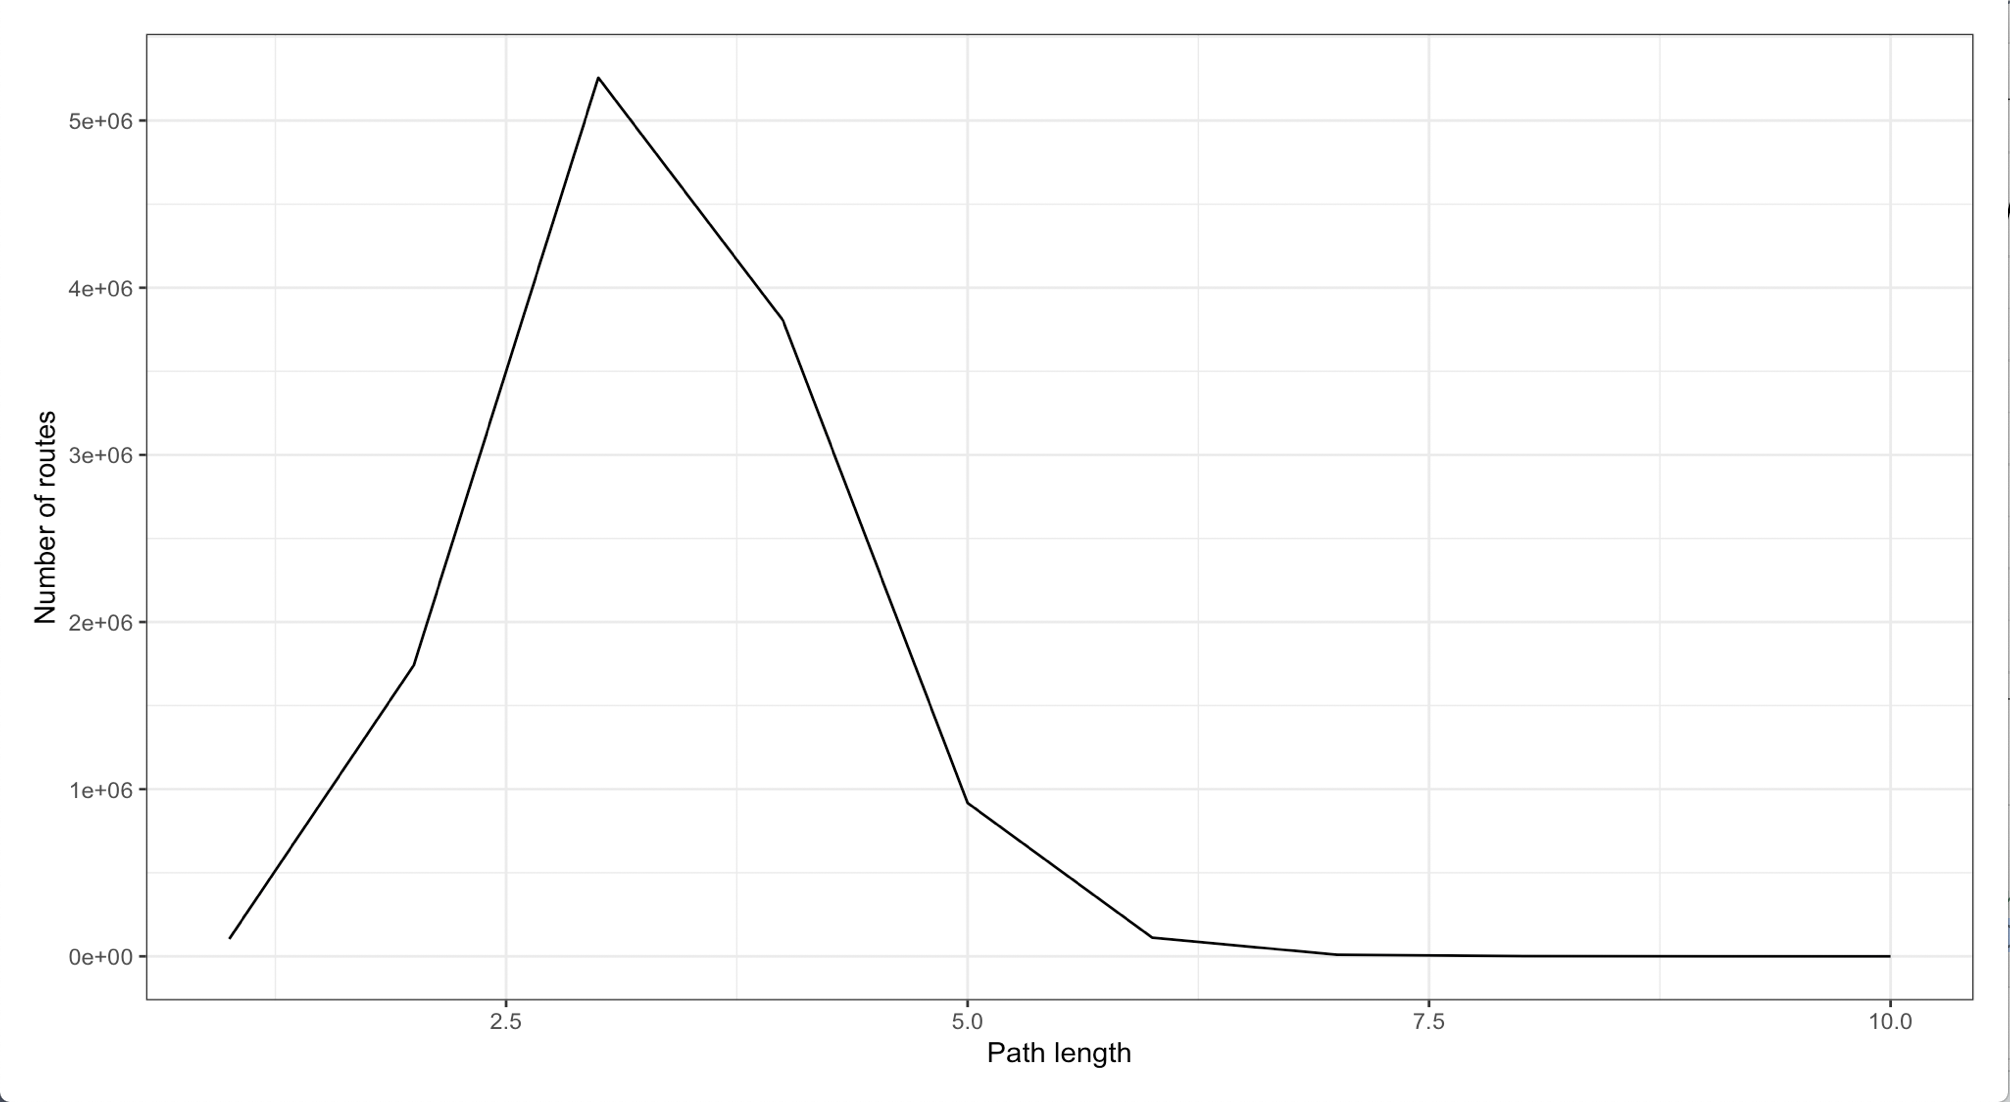
\includegraphics[width=11cm, height=7cm]{figures/path_len.png}
\centering
\end{figure}

Again, what do you think we can learn based on what we know about Wiki degree? And how would you go about computing average path length?

\section{Single source shortest path and applications}

One very common application of graphs is the single source shortest path problem. Google Maps provides just one of countless many of such applications.

In the realm of undirected graphs, the algorithm to compute shortest path uses a well-known graph algorithm called breadth-first search, a.k.a. BFS. An implementation is as follows:

\begin{itemize}
    \item init all nodes to be infinitely far away, except for source at distance = 0
    \item init current boundary to be source node
    \item while boundary not empty
    \begin{itemize}
        \item create empty list for new boundary
        \item for all nodes in current boundary
        \begin{itemize}
            \item loop over undiscovered neighbors
            \item set neighbors distance = current distance + 1
            \item add neighbor to next boundary
        \end{itemize}
    \end{itemize}
\end{itemize}

See if you can implement this algorithm in R.

The algorithm finds many more applications outside of maps and navigation. For example, let's say that you wanted to find out how many distinct groups of friends there were on a social network. This is an application of connected components, which may efficiently rely on BFS to generate the correct result (one savvy classmate suggested another efficient solution making use of the union find data structure, but that's beyond the scope of this course).

\section{Mutual friends and counting triangles}

The final application of graphs we'll look at is counting mutual friends. In a social network, for example, we are often interested in how many friends of friends are also friends.

We can use the following pseudo-code to implement the algorithm:

\begin{itemize}
    \item For all nodes in the graph
    \begin{itemize}
        \item Compute its neighbors
        \item For each unique pair in the neighbors list (pairwise generation)
        \begin{itemize}
            \item Increment the number of mutual friends between the nodes in the pair by 1 since they have the the original node in common (would require a matrix to compute)
        \end{itemize}
    \end{itemize}
\end{itemize}

Using a variant of this algorithm, one can also compute the number of 3-friend groups aka triangles (can you write the pseudocode for this?).

On a side note, around this time, the question came up regarding whether an adjacency list was really constant, or O(1), access time considering some nodes may be adjacent to multiple nodes and iterating through the list would take a long time. In the naive implementation where only the nodes are hashed to a list of adjacent nodes, then there would be a slight load factor added onto the running time, though assuming very few nodes would have a large degree, the load factor would be negligible. If you absolutely needed a smarter adjacency list representation, there are ways to do it. Those, however, are beyond the scope of this lecture.

\section{The fallacy of causation}

Time and time again, we always say: correlation (or prediction) does not imply causation, yet this happens far too often the scientific world because it is so easy to make this mistake.

Prediction: make a forecast but assuming the universe stays as it is
Causation: anticipating what will happen when the universe changes

Before moving on, it is important that we ask the right questions. It is far too tempting to ask reverse causal inference questions such as:

\begin{itemize}
    \item What makes an email spam?
    \item What caused my kid to get sick?
    \item Why did the stock market drop?
\end{itemize}

The problem is that these questions are very difficult to answer. It is better to ask forward causal inference questions such as:

\begin{itemize}
    \item How does education impact future earnings?
    \item What is the effect of advertising on sales?
    \item How does hospitalization affect health?
\end{itemize}

These are still hard questions, but they are far less contentious. With enough data, conclusions can be more easily drawn. This does not mean, however, that we can let our guard down.

\section{A simple example}

Consider the last question: How does hospitalization affect health?

Suppose someone claimed that if a patient visited the hospital today, they would be healthy tomorrow. What's wrong with this claim?

\begin{figure}[H]
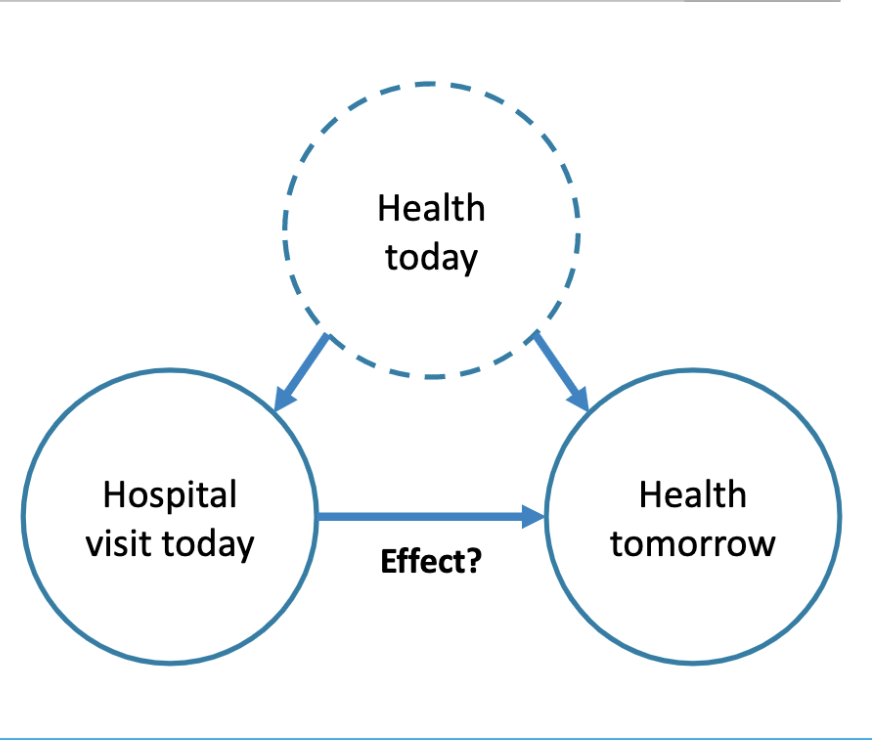
\includegraphics[width=6cm, height=6cm]{figures/health.png}
\centering
\end{figure}

When someone makes a blanket causation statement like this, they ignore factors called confounds which might literally be be changing together with the implied cause. In this case, said person ignores the fact that a person's health today likely influences their health tomorrow. Therefore, since we're observing both the patient's hospital visit status AND their health today, we cannot make any causation claim.

To put it mathematically, the causal effect we're trying to measure is:

\[\Delta_{obs} = s_{hospital} - s_{home}\]

where $$s_{hospital}$$ is the number of patients that were sick and went to the hospital and $$s_{home}$$ is the number of patients that were sick and stayed home. In an ideal world, this would be the only thing we would be measuring. Unfortunately, we must take into account the confounding factor. In this case, assuming that all healthy people stay home and sick people go to the hospital in our dataset, we actually have that:

\[\Delta_{obs} = (s_{hospital} - s_{home}) - (s_{home} - h_{home})\]

where we introduce the selection bias term (the latter) and a new variable, $$h_{home}$$, which indicates the number of healthy people that stayed home. This term is in practice quite difficult to calculate and will often be negative, meaning that without the selection bias term, we could be massively underestimating.

In summary, the observed difference equation:

\[\Delta_{obs} = obs - bias\]

The nightmarish situation in terms of selection bias is Simpson's paradox, in which selection bias can be so large that the observational and causal estimates give opposite effect. Consider, for instance, this:

\begin{figure}[H]
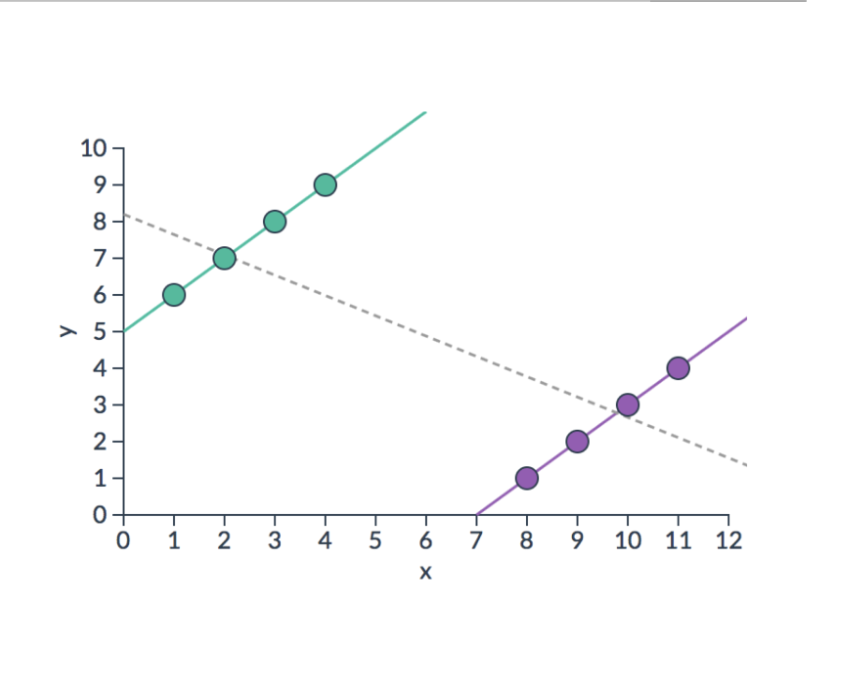
\includegraphics[width=6cm, height=6cm]{figures/simpson.png}
\centering
\end{figure}

The two colored trend lines are what we should be fitting since they are isolated. However, if we didn't take into account selection bias, we would attempt to fit a regression line onto both sets of data, evidence by the dotted line. This naive regression, in effect, would tell us that going to hospitals makes you less healthy (see what I've been telling you y'all, the government is secretly making y'all sick, I don't need no hospitals!).

\section{Dealing with confounds}

The way we do this is to change one and only one thing, then compare outcomes. We can only estimate what would have happened if we did something else.

We can use random assignment to create two groups that differ only in what they receive.

\end

\end{document}

%%% Local Variables:
%%% mode: latex
%%% TeX-master: t
%%% End:
